%============================================================
%  CASH FLOW FORECASTING & VARIANCE ANALYSIS PROPOSAL
%  COB Solutions → PT of the City
%  Author: Abdelrahman Hamdy — COB Solutions
%  Compile: pdflatex x2
%============================================================
\documentclass[11pt,a4paper]{article}

\usepackage[T1]{fontenc}
\usepackage[utf8]{inputenc}
\usepackage{mathptmx}
\usepackage[scaled=0.92]{helvet}
\usepackage{courier}
\usepackage{microtype}
\usepackage[top=2.5cm,bottom=2.5cm,left=2.5cm,right=2.5cm,headheight=16pt]{geometry}
\usepackage{xcolor}
\usepackage{graphicx}
\usepackage{amsmath}
\usepackage{booktabs}
\usepackage{array}
\usepackage{colortbl}
\usepackage{multicol}
\usepackage{enumitem}
\usepackage{fancyhdr}
\usepackage{titlesec}
\usepackage{tcolorbox}
\usepackage{tikz}
\usepackage{hyperref}
\usepackage{tabularx}

\usetikzlibrary{shapes.geometric,arrows.meta,positioning,fit,calc,shadows,backgrounds}
\tcbuselibrary{skins,breakable}

%-----------------------------------------------------------
% COLOURS
%-----------------------------------------------------------
\definecolor{PrimaryBlue}{HTML}{1A3C5E}
\definecolor{AccentTeal}{HTML}{0D7C8C}
\definecolor{AccentGold}{HTML}{C8962A}
\definecolor{LightBg}{HTML}{F4F7FA}
\definecolor{MidGray}{HTML}{6B7B8D}
\definecolor{DangerRed}{HTML}{C0392B}
\definecolor{SuccessGreen}{HTML}{1E8449}
\definecolor{WarningAmber}{HTML}{D4850A}
\definecolor{SoftBlue}{HTML}{D6E4F0}
\definecolor{SoftTeal}{HTML}{D0EEF2}
\definecolor{SoftGold}{HTML}{FAF0DC}
\definecolor{SoftRed}{HTML}{FADBD8}
\definecolor{SoftGreen}{HTML}{D5F5E3}
\definecolor{TableHead}{HTML}{1A3C5E}
\definecolor{TableAlt}{HTML}{EAF2FA}
\definecolor{RuleColor}{HTML}{B0C4D8}

%-----------------------------------------------------------
% HYPERREF
%-----------------------------------------------------------
\hypersetup{colorlinks=true,linkcolor=PrimaryBlue,urlcolor=AccentTeal,
  pdftitle={Cash Flow Forecasting \& Variance Analysis --- COB Solutions},
  bookmarksnumbered=true}

%-----------------------------------------------------------
% HEADER / FOOTER
%-----------------------------------------------------------
\pagestyle{fancy}\fancyhf{}
\fancyhead[L]{\color{MidGray}\small\textit{COB Solutions --- Prepared for PT of the City}}
\fancyfoot[C]{\color{MidGray}\thepage}
\renewcommand{\headrulewidth}{0.4pt}
\renewcommand{\headrule}{\hbox to\headwidth{\color{RuleColor}\leaders\hrule height\headrulewidth\hfill}}

%-----------------------------------------------------------
% SECTION STYLING
%-----------------------------------------------------------
\titleformat{\section}{\color{PrimaryBlue}\Large\bfseries}
  {\colorbox{PrimaryBlue}{\color{white}\ \thesection\ }}{0.8em}{}
  [\vspace{-0.2em}\color{RuleColor}\rule{\linewidth}{1.5pt}\vspace{0.3em}]
\titleformat{\subsection}{\color{AccentTeal}\large\bfseries}
  {\color{AccentTeal}\thesubsection}{0.6em}{}
  [\vspace{-0.3em}\color{RuleColor}\rule{\linewidth}{0.6pt}]
\titleformat{\subsubsection}{\color{PrimaryBlue}\normalsize\bfseries}
  {\color{AccentGold}\thesubsubsection}{0.5em}{}
\titlespacing*{\section}{0pt}{1.6em}{0.8em}
\titlespacing*{\subsection}{0pt}{1.2em}{0.5em}
\titlespacing*{\subsubsection}{0pt}{0.9em}{0.3em}

%-----------------------------------------------------------
% LISTS
%-----------------------------------------------------------
\setlist[itemize,1]{label={\color{AccentTeal}\textbullet},leftmargin=1.5em,itemsep=0.25em,topsep=0.3em}
\setlist[itemize,2]{label={\color{AccentGold}\small$\blacktriangleright$},leftmargin=1.5em,itemsep=0.15em}
\setlist[enumerate,1]{label={\color{PrimaryBlue}\bfseries\arabic*.},leftmargin=1.8em,itemsep=0.25em}

%-----------------------------------------------------------
% TCOLORBOX STYLES
%-----------------------------------------------------------
\tcbset{
  infobox/.style={enhanced,breakable,colback=SoftBlue,colframe=PrimaryBlue,
    boxrule=1.2pt,arc=4pt,left=8pt,right=8pt,top=6pt,bottom=6pt,
    fonttitle=\bfseries\color{white},
    attach boxed title to top left={yshift=-2mm,xshift=6mm},
    boxed title style={colback=PrimaryBlue,arc=3pt,boxrule=0pt}},
  warnbox/.style={enhanced,breakable,colback=SoftGold,colframe=WarningAmber,
    boxrule=1.2pt,arc=4pt,left=8pt,right=8pt,top=6pt,bottom=6pt,
    fonttitle=\bfseries\color{white},
    attach boxed title to top left={yshift=-2mm,xshift=6mm},
    boxed title style={colback=WarningAmber,arc=3pt,boxrule=0pt}},
  successbox/.style={enhanced,breakable,colback=SoftGreen,colframe=SuccessGreen,
    boxrule=1.2pt,arc=4pt,left=8pt,right=8pt,top=6pt,bottom=6pt,
    fonttitle=\bfseries\color{white},
    attach boxed title to top left={yshift=-2mm,xshift=6mm},
    boxed title style={colback=SuccessGreen,arc=3pt,boxrule=0pt}},
  statbox/.style={enhanced,colback=LightBg,colframe=AccentGold,
    boxrule=2pt,arc=6pt,left=10pt,right=10pt,top=8pt,bottom=8pt},
  rulebox/.style={enhanced,breakable,colback=LightBg,colframe=PrimaryBlue,
    boxrule=0.8pt,arc=3pt,left=7pt,right=7pt,top=6pt,bottom=6pt,
    borderline west={3pt}{0pt}{AccentTeal}}
}

%-----------------------------------------------------------
% TIKZ BASE STYLES
%-----------------------------------------------------------
\tikzset{
  FB/.style={rectangle,rounded corners=3pt,
             minimum width=2.4cm,minimum height=0.85cm,
             text centered,align=center,draw,thick,
             font=\footnotesize\bfseries},
  arr/.style={-{Stealth[length=4.5pt]},thick},
  nB/.style={FB,fill=SoftBlue, draw=PrimaryBlue,text=PrimaryBlue},
  nT/.style={FB,fill=SoftTeal, draw=AccentTeal, text=AccentTeal},
  nG/.style={FB,fill=SoftGold, draw=AccentGold, text=AccentGold},
  nV/.style={FB,fill=SoftGreen,draw=SuccessGreen,text=SuccessGreen},
  nR/.style={FB,fill=SoftRed,  draw=DangerRed,  text=DangerRed}
}

%-----------------------------------------------------------
% HELPERS
%-----------------------------------------------------------
\newcolumntype{L}[1]{>{\raggedright\arraybackslash}p{#1}}
\newcolumntype{C}[1]{>{\centering\arraybackslash}p{#1}}

%============================================================
\begin{document}
%============================================================

%------------------------------------------------------------
% COVER PAGE
%------------------------------------------------------------
\begin{titlepage}
\pagecolor{PrimaryBlue}\color{white}
\vspace*{0.6cm}
\begin{center}
  \textcolor{AccentGold}{\rule{0.88\linewidth}{2pt}}\\[0.3em]
  \textcolor{AccentGold}{\rule{0.88\linewidth}{0.5pt}}\\[1.4cm]

  {\fontsize{14}{18}\selectfont\color{SoftBlue}\textsc{COB Solutions}}\\[0.4em]
  {\fontsize{12}{16}\selectfont\color{AccentGold}\textbf{Prepared for PT of the City}}\\[1.2cm]

  {\fontsize{28}{36}\selectfont\bfseries Strategic Proposal}\\[0.3em]
  {\fontsize{20}{28}\selectfont\bfseries Predictive Cash Flow \&}\\[0.1em]
  {\fontsize{20}{28}\selectfont\bfseries Financial Intelligence Framework}\\[0.8em]

  \textcolor{AccentGold}{\rule{0.5\linewidth}{0.8pt}}\\[0.6em]
  {\color{SoftBlue}\small
    Revenue Cycle Optimization \textbullet{} Variance Analysis \textbullet{}
    Operational Accountability \textbullet{} RCM Intelligence}\\[2.0cm]


  \vfill
  \textcolor{AccentGold}{\rule{0.88\linewidth}{0.5pt}}\\[0.3em]
  \textcolor{AccentGold}{\rule{0.88\linewidth}{2pt}}
\end{center}
\end{titlepage}
\nopagecolor\color{black}

%------------------------------------------------------------
% TABLE OF CONTENTS
%------------------------------------------------------------
\newpage
\tableofcontents
\newpage

%============================================================
\section{Executive Summary}
%============================================================

This proposal responds to the strategic initiative defined by \textbf{Mr.\ Moustafa Ezz},
Finance Manager and project owner at PT of the City. Mr.\ Ezz has identified a critical
gap between submitted claims and actual banked cash, and between departmental budgets
and measurable operational output. \textbf{COB Solutions} proposes a unified financial
intelligence framework that closes these gaps through predictive forecasting, rigorous
variance analysis, and operational accountability.

PT of the City operates a complex Revenue Cycle Management (RCM) environment spanning
lead generation, clinical documentation, authorization, billing, and clearinghouse
submission. Current reporting relies heavily on gross submission volumes and static
estimates. This creates inflated liquidity expectations, delayed corrective action, and
limited visibility into \emph{where} revenue is lost and \emph{who} is accountable.

COB Solutions will deliver an intelligent RCM and financial model with three interconnected
objectives:

\begin{enumerate}
  \item \textbf{Predictive Cash Inflow} --- Move from static estimates to a mature forecasting
        model targeting \textbf{98\% liquidity accuracy}, accounting for denial rates,
        correction cycles, and insurance-specific payment behavior.
  \item \textbf{Variance Analysis \& Accountability} --- Compare the Master Budget against
        actuals using a \textbf{Sales vs.\ Budget} framework
        that rewards genuine performance and flags underinvestment disguised as savings.
  \item \textbf{Operational Governance} --- Protect automation gains through administration
        logs, audit trails, and a formal COB Solutions engagement model with documented
        milestones.
\end{enumerate}

\begin{tcolorbox}[statbox]
\begin{center}
  \Large\bfseries\color{PrimaryBlue}Strategic Outcomes\\[0.5em]
\end{center}
\vspace{0.2em}
\begin{center}
\begin{tabularx}{0.96\linewidth}{C{3.0cm} C{3.0cm} C{3.0cm} C{3.0cm}}
  \textcolor{PrimaryBlue}{\bfseries Predictability} &
  \textcolor{AccentTeal}{\bfseries Accountability} &
  \textcolor{AccentGold}{\bfseries Visibility} &
  \textcolor{SuccessGreen}{\bfseries Revenue Protection} \\[0.3em]
  \small Know exact cash &
  \small Hold departments to budget \& KPIs &
  \small Pinpoint clinic-level gaps &
  \small Minimize denial leakage \\
\end{tabularx}
\end{center}
\end{tcolorbox}

\begin{tcolorbox}[rulebox,title={The ``So What?''}]
Financial reporting must answer more than ``what was submitted.'' It must answer
\emph{what will actually arrive in the bank} and \emph{which department or clinic cluster
is responsible} when expectations are not met. This proposal transforms that question
from a retrospective report into an active management tool.
\end{tcolorbox}


%============================================================
\section{Strategic Context \& Current State}
%============================================================

\subsection{The RCM Visibility Challenge}

Optimizing cash flow requires end-to-end mapping of every RCM touchpoint---from initial
lead generation through clinical documentation, authorization, billing release, and
final claim submission via Waystar. Without this visibility, leadership cannot distinguish
systemic bottlenecks from isolated errors, and corrective action remains broad and inefficient.

The current investigative phase includes a collaborative review with the Authorization and
Billing teams, including analysis of rejected claims. By auditing denial instances,
COB Solutions will document primary rejection triggers and build a structured database of
common errors---establishing the baseline required for denial prediction and root-cause
accountability.

\subsection{Automation Progress}

PT of the City is transitioning from manual entry workflows to automated billing through
WebPT and Waystar. The impact is substantial and must be reflected in any forecasting model:

\begin{center}
\begin{tabularx}{0.92\linewidth}{L{4.2cm} C{2.8cm} X}
  \rowcolor{TableHead}
  \color{white}\textbf{Metric} & \color{white}\textbf{Before} & \color{white}\textbf{Current State} \\
  Auto-processed claims     & Manual line-by-line entry  & \textbf{70\%} routed automatically by insurance rules \\
  \rowcolor{TableAlt}
  Human intervention        & All claims                 & \textbf{30\%} exceptions (e.g.\ Medicare, Workers' Comp) \\
\end{tabularx}
\end{center}

These gains are only sustainable if protected by administration logs and audit trails---a
core component of this proposal (Section~\ref{sec:governance}).

\subsection{RCM Process Mapping}

Accurate forecasting depends on understanding how claims move through PT of the City's
operational environment. During the Discovery phase, COB Solutions will map the full RCM
cycle in partnership with PT of the City's operational leadership. \textbf{Dr.\ Adnan},
Business Developer, brings the deepest practical knowledge of the organization's RCM cycle
and will serve as the primary domain advisor during process mapping---ensuring the model
reflects real-world workflows rather than theoretical assumptions.


%============================================================
\section{Proposed Solution}
%============================================================

COB Solutions proposes a six-pillar framework that integrates cash inflow forecasting,
denial management, expense variance analysis, clinical cost tracking, future revenue
readiness, and system governance into a single financial intelligence platform.

%------------------------------------------------------------
\subsection{Pillar A --- Predictive Cash Inflow Forecasting}
%------------------------------------------------------------

The financial strategy must shift from static forecasting to a \textbf{mature predictive
model}. Rather than treating gross submitted claims as expected revenue, the model applies
historical patterns to produce a net cash forecast aligned with actual banking outcomes.

\begin{tcolorbox}[infobox,title={How the Mature Model Works}]
If \$X is submitted in claims, historical analysis may indicate that approximately
10\% will be rejected. Rather than forecasting the full \$X in the current cycle, the
model \textbf{deducts} the rejected portion from near-term expectations and \textbf{shifts}
it forward to a subsequent forecast period to account for correction and resubmission. The cash-on-hand
forecast therefore reflects what will actually arrive---not what was submitted.
\end{tcolorbox}

\subsubsection{Core Capabilities}

\begin{itemize}
  \item \textbf{Intelligent Forecasting} --- Project cash inflow based on submitted claims,
        company SLAs, and insurance-specific payment behavior patterns.
  \item \textbf{Denial Prediction} --- Estimate dollar amounts likely to be denied before
        they occur, using historical rejection rates and categorized denial data.
  \item \textbf{Forecast Adjustments} --- Automatically shift rejected amounts to future
        forecast periods based on the standard correction and resubmission cycle.
  \item \textbf{Success vs.\ Delay Tracking} --- Maintain an 80\% baseline for claims paid
        on first submission; track and decompose the remaining 20\% by root cause.
\end{itemize}

\subsubsection{Forecasting Factor Impact}

\begin{center}
\begin{tabularx}{\linewidth}{L{3.2cm} X L{4.5cm}}
  \rowcolor{TableHead}
  \color{white}\textbf{Factor} & \color{white}\textbf{Description} & \color{white}\textbf{Liquidity Impact} \\
  Success Rate &
    Base expectation for successful claims &
    Target: \textbf{80\%} paid on first submission \\
  \rowcolor{TableAlt}
  Medical Auditing Delays &
    Failure to close clinical notes promptly &
    Estimated \textbf{5\%} delay in submission volume \\
  Authorization / Checks &
    Missing benefit verification or authorization errors &
    Estimated \textbf{5\%} delay; manual intervention required \\
  \rowcolor{TableAlt}
  Coding Errors &
    Missing CPT codes or incorrect diagnoses &
    Immediate rejection on clearinghouse platforms \\
  Correction Cycles &
    Fix-and-resubmit window for denied claims &
    Shifts \textbf{10--20\%} of expected cash flow to a subsequent period \\
\end{tabularx}
\end{center}

%------------------------------------------------------------
\subsection{Pillar B --- Denial Management \& Department Accountability}
%------------------------------------------------------------

Denial data becomes actionable only when categorized with sufficient granularity to drive
corrective action at the clinic and department level.

\begin{itemize}
  \item \textbf{Categorization} --- Denials indexed by clinic, patient, and specific reason
        to pinpoint operational gaps.
  \item \textbf{Error Source Identification} --- Distinguish Front Desk errors (e.g.\ incorrect
        patient names) from Medical Auditing errors (e.g.\ wrong CPT or modifier codes) and
        Authorization errors (e.g.\ missing benefit verification).
  \item \textbf{Clinic-Cluster Reporting} --- Enable leadership to determine whether a specific
        clinic or cluster underperforms due to administrative errors or clinical documentation
        gaps.
\end{itemize}

\begin{tcolorbox}[warnbox,title={Operational Principle}]
Every denial has an owner. The framework does not stop at reporting rejection volume---it
assigns accountability to the function responsible, enabling targeted intervention rather
than organization-wide policy changes.
\end{tcolorbox}

%------------------------------------------------------------
\subsection{Pillar C --- Cash Outflow \& Variance Analysis}
%------------------------------------------------------------

Strategic variance analysis is the primary mechanism for maintaining departmental
accountability across PT of the City.

\subsubsection{Master Budget vs.\ Actuals}

The \textbf{Master Budget} is established with built-in volume assumptions that reflect
expected operational patterns. Actuals are compared against this baseline not merely for
tracking, but as the foundation for performance evaluation and corrective action.

\subsubsection{Sales vs.\ Budget --- The Accountability Framework}

\begin{center}
\begin{tabularx}{0.92\linewidth}{L{3.5cm} X}
  \rowcolor{TableHead}
  \color{white}\textbf{Performance} & \color{white}\textbf{Organizational Response} \\
  \cellcolor{SoftGreen}\textbf{Overperformance} &
    Departments exceeding sales targets while remaining within expense budget are eligible
    for performance bonuses and formal recognition. \\
  \rowcolor{TableAlt}
  \cellcolor{SoftRed}\textbf{Underperformance} &
    Departments falling below budget targets trigger corrective review to identify root
    causes---whether insufficient patient volume, operational inefficiency, or process failure. \\
\end{tabularx}
\end{center}

\subsubsection{The Commercial Department Rule}

Staying under the expense budget is \textbf{not} success if sales targets are not met.
If a department spends only 3\% of its 5\% budget allocation but fails to generate the
required patient leads, that ``saving'' is classified as a \textbf{failure of investment},
not an efficiency gain. True performance requires simultaneous optimization of spend and output.

\subsubsection{Three-Pillar Department Evaluation}

Every department will be evaluated on three interconnected dimensions:

\begin{center}
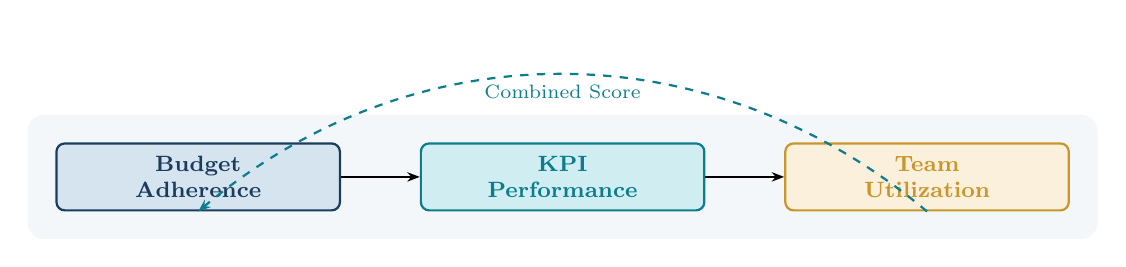
\begin{tikzpicture}[node distance=0.6cm and 1.0cm]
  \node[nB,minimum width=3.6cm] (budget) {Budget\\Adherence};
  \node[nT,minimum width=3.6cm,right=1.0cm of budget] (kpi) {KPI\\Performance};
  \node[nG,minimum width=3.6cm,right=1.0cm of kpi] (util) {Team\\Utilization};
  \draw[arr](budget)--(kpi);
  \draw[arr](kpi)--(util);
  \draw[arr,dashed,AccentTeal](util.south) to[bend right=40]
    node[below,font=\scriptsize\color{MidGray}]{Combined Score} (budget.south);
  \begin{scope}[on background layer]
    \node[fill=LightBg,rounded corners=6pt,inner sep=10pt,
          fit=(budget)(kpi)(util)] {};
  \end{scope}
\end{tikzpicture}
\end{center}

Departmental expenditure will be strictly evaluated---for example, ensuring the Commercial
team adheres to its allocated percentage of total revenue (typically 6--7\%).


%------------------------------------------------------------
\subsection{Pillar D --- Clinical COGS \& Utility Allocation}
%------------------------------------------------------------

In a physical therapy context, the Cost of Revenue (COGS) represents the direct costs
required to treat a patient. Efficiently managing the COGS ratio---targeting approximately
\textbf{50\% of revenue}---is essential for maintaining healthy profit margins.

\subsubsection{Four Components of Clinical COGS}

\begin{enumerate}
  \item \textbf{Labor Hours} --- Direct cost of clinical staff delivering patient treatment.
  \item \textbf{Clinical Supplies} --- Materials consumed during treatment sessions.
  \item \textbf{Direct Utilities} --- Electricity and climate control required for functional
        treatment rooms.
  \item \textbf{Clinical Documentation} --- Costs associated with Medical Auditing and CVI
        teams who close clinical notes to enable billing.
\end{enumerate}

\subsubsection{Utility Allocation Logic}

A specialized \textbf{40/60 or 70/30} split separates COGS from Overhead:

\begin{itemize}
  \item \textbf{COGS} --- Treatment room lighting and air conditioning. A patient would
        likely refuse treatment if the room were too hot or dark; these costs directly
        enable revenue-generating activity.
  \item \textbf{Overhead} --- Corridor lighting, kitchen utilities, and shared spaces whose
        absence would not strictly prevent a clinician from seeing a patient.
\end{itemize}

Accurate COGS allocation is vital as PT of the City prepares for diagnostic service expansion.


%------------------------------------------------------------
\subsection{Pillar E --- Future Revenue Integration}
%------------------------------------------------------------

PT of the City is diversifying revenue through an upcoming pipeline of specialized
diagnostic services---higher barriers to entry and higher revenue potential than standard
physical therapy. Planned areas include:

\begin{multicols}{2}
\begin{itemize}
  \item Nerve Conduction Tests
  \item Lymphedema Management
  \item Orthopedic Specializations
  \item Pelvic Health
\end{itemize}
\end{multicols}

To mitigate the cost of hiring external specialists immediately, existing medical staff
are undergoing internal certification training---a strategic cost-saving approach. Once
operational, these revenue streams must be fully integrated into the automated billing
architecture to prevent new manual bottlenecks. COB Solutions will ensure the forecasting
and variance framework accommodates new service lines from launch.


%------------------------------------------------------------
\subsection{Pillar F --- System Governance \& Audit Trails}
\label{sec:governance}
%------------------------------------------------------------

Automation gains are only as durable as the controls that protect them.

\begin{itemize}
  \item \textbf{Administration Logs} --- Every system action recorded with User and Action.
        Mandatory for performance monitoring and as a preventative security measure
        against unauthorized deletions or data corruption.
  \item \textbf{Audit Trails} --- Full traceability of who entered, modified, or deleted
        billing and financial data.
  \item \textbf{Utilization Monitoring} --- Ensure billing agents actively and correctly
        leverage WebPT/Waystar automation rather than reverting to manual workarounds.
\end{itemize}

\subsubsection{COB Solutions Engagement Model}

COB Solutions operates as an external service provider to PT of the City. All new scope
beyond this proposal requires a formal \textbf{Engagement Letter} with SLA-based deposits
and documented milestones---ensuring every feature is properly scoped, funded, and delivered.


%============================================================
\section{Architecture Overview}
%============================================================

The following diagram illustrates how data inputs flow through the intelligence layer
to produce leadership-ready outputs. This is a managerial view; technical implementation
details will be documented during Phase~1.

\vspace{0.5em}
\begin{center}
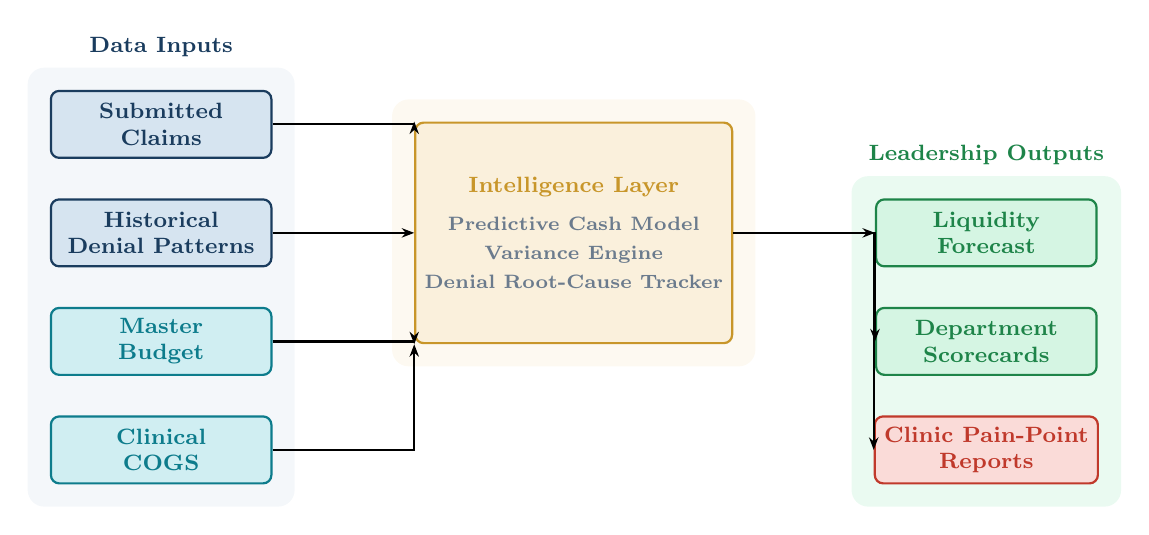
\begin{tikzpicture}[node distance=0.55cm and 0.5cm,every node/.style={align=center,font=\scriptsize\bfseries}]

  % Inputs
  \node[nB,minimum width=2.8cm] (claims) {Submitted\\Claims};
  \node[nB,minimum width=2.8cm,below=0.5cm of claims] (hist) {Historical\\Denial Patterns};
  \node[nT,minimum width=2.8cm,below=0.5cm of hist] (budget) {Master\\Budget};
  \node[nT,minimum width=2.8cm,below=0.5cm of budget] (cogs) {Clinical\\COGS};

  % Engine
  \node[nG,minimum width=3.2cm,minimum height=2.8cm,right=1.8cm of hist] (engine) {
    \vspace{0.2em}Intelligence Layer\\[0.4em]
    {\scriptsize\color{MidGray}Predictive Cash Model}\\[0.1em]
    {\scriptsize\color{MidGray}Variance Engine}\\[0.1em]
    {\scriptsize\color{MidGray}Denial Root-Cause Tracker}
  };

  % Outputs
  \node[nV,minimum width=2.8cm,right=1.8cm of engine] (daily) {Liquidity\\Forecast};
  \node[nV,minimum width=2.8cm,below=0.5cm of daily] (score) {Department\\Scorecards};
  \node[nR,minimum width=2.8cm,below=0.5cm of score] (pain) {Clinic Pain-Point\\Reports};

  \draw[arr](claims.east)-|(engine.north west);
  \draw[arr](hist.east)--(engine.west);
  \draw[arr](budget.east)-|(engine.south west);
  \draw[arr](cogs.east)-|(engine.south west);
  \draw[arr](engine.east)--(daily.west);
  \draw[arr](engine.east)-|(score.west);
  \draw[arr](engine.east)-|(pain.west);

  \node[font=\footnotesize\bfseries\color{PrimaryBlue},above=0.3cm of claims] {Data Inputs};
  \node[font=\footnotesize\bfseries\color{SuccessGreen},above=0.3cm of daily] {Leadership Outputs};

  \begin{scope}[on background layer]
    \node[fill=LightBg,rounded corners=6pt,inner sep=8pt,
          fit=(claims)(cogs)] {};
    \node[fill=SoftGold!40,rounded corners=6pt,inner sep=8pt,
          fit=(engine)] {};
    \node[fill=SoftGreen!50,rounded corners=6pt,inner sep=8pt,
          fit=(daily)(pain)] {};
  \end{scope}
\end{tikzpicture}
\end{center}

%============================================================
\section{Phased Implementation Roadmap}
%============================================================

COB Solutions recommends a four-phase delivery approach. Each phase concludes with a
\textbf{go/no-go checkpoint} requiring sign-off from \textbf{Mr.\ Moustafa Ezz} as project
owner before proceeding.

\vspace{0.5em}
\begin{center}
\begin{tabularx}{\linewidth}{L{4.5cm} X}
  \rowcolor{TableHead}
  \color{white}\textbf{Phase} & \color{white}\textbf{Outcome} \\
  Phase 1 --- Discovery \& Baseline &
    Data foundation and RCM map complete \\
  \rowcolor{TableAlt}
  Phase 2 --- Pilot &
    Forecasting model validated on pilot clinics \\
  Phase 3 --- Full Rollout &
    Organization-wide dashboards live \\
  \rowcolor{TableAlt}
  Phase 4 --- Expansion Readiness &
    New revenue streams and governance controls ready \\
\end{tabularx}
\end{center}

\vspace{0.5em}
\begin{center}
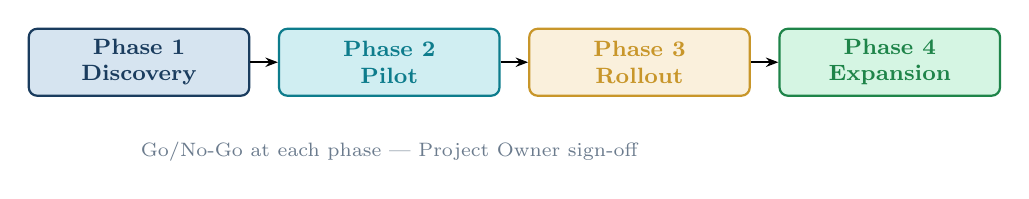
\begin{tikzpicture}[node distance=0.4cm and 0.35cm,every node/.style={align=center,font=\scriptsize\bfseries}]
  \node[nB,minimum width=2.8cm] (p1) {Phase 1\\Discovery};
  \node[nT,minimum width=2.8cm,right=0.35cm of p1] (p2) {Phase 2\\Pilot};
  \node[nG,minimum width=2.8cm,right=0.35cm of p2] (p3) {Phase 3\\Rollout};
  \node[nV,minimum width=2.8cm,right=0.35cm of p3] (p4) {Phase 4\\Expansion};
  \draw[arr](p1)--(p2);
  \draw[arr](p2)--(p3);
  \draw[arr](p3)--(p4);
  \node[below=0.45cm of p2,font=\scriptsize\color{MidGray}] {Go/No-Go at each phase --- Project Owner sign-off};
\end{tikzpicture}
\end{center}

%------------------------------------------------------------
\subsection{Phase 1 --- Discovery \& Baseline}
%------------------------------------------------------------

\textbf{Objective:} Establish the data foundation and operational baseline required
for accurate forecasting.

\begin{tcolorbox}[infobox,title={Activities}]
\begin{itemize}
  \item \textbf{Data ingestion} --- Connect and validate billing exports from WebPT/Waystar,
        rejected-claims history, and Master Budget files provided by Finance.
  \item \textbf{Denial audit} --- Analyze rejected claims; classify primary denial
        triggers (coding, authorization, documentation, front-desk errors) and build the
        initial denial trigger database.
  \item \textbf{RCM process mapping} --- Document the end-to-end claim journey (lead intake
        through submission) with Dr.\ Adnan to ensure the model reflects actual workflows.
  \item \textbf{Historical pattern analysis} --- Calculate baseline success rates, average
        payment cycles, and rejection percentages by payer and clinic cluster.
  \item \textbf{Baseline accuracy score} --- Measure current forecast error (submitted claims
        vs.\ actual banked cash) to establish the starting point before model deployment.
\end{itemize}
\end{tcolorbox}

\textbf{Deliverables:} Denial trigger database \textbullet{} RCM process map
\textbullet{} Data integration report \textbullet{} Baseline forecast accuracy score

%------------------------------------------------------------
\subsection{Phase 2 --- Pilot}
%------------------------------------------------------------

\textbf{Objective:} Validate the predictive cash-inflow model on a controlled subset before
organization-wide deployment.

\begin{tcolorbox}[infobox,title={Activities}]
\begin{itemize}
  \item \textbf{Pilot clinic selection} --- Deploy on 2--3 clinic clusters with Mr.\ Ezz's
        approval; prioritize clusters with representative denial volume and payer mix.
  \item \textbf{Cash-inflow model v1} --- Build the mature forecasting engine: apply historical
        denial rates, shift rejected amounts to subsequent forecast periods, and produce
        net cash projections.
  \item \textbf{Root-cause delay tracker} --- Decompose the 20\% delayed claims by source
        (Medical Auditing, Authorization, Front Desk, coding) for pilot clinics.
  \item \textbf{Variance dashboard v1} --- Compare Master Budget vs.\ actuals for
        pilot scope; implement Sales vs.\ Budget over/underperformance flags.
  \item \textbf{Pilot review session} --- Present accuracy results to Mr.\ Ezz; refine model
        parameters based on feedback before full rollout.
\end{itemize}
\end{tcolorbox}

\textbf{Deliverables:} Forecast report (pilot clinics) \textbullet{}
Root-cause delay breakdown \textbullet{} Variance dashboard v1 \textbullet{}
Pilot accuracy score vs.\ 98\% target

%------------------------------------------------------------
\subsection{Phase 3 --- Full Rollout}
%------------------------------------------------------------

\textbf{Objective:} Extend validated models to all clinics and activate full financial
intelligence capabilities.

\begin{tcolorbox}[infobox,title={Activities}]
\begin{itemize}
  \item \textbf{Organization-wide deployment} --- Roll out the cash-inflow model and denial
        categorization to all clinic locations.
  \item \textbf{COGS module} --- Integrate clinical Cost of Revenue tracking: labor hours,
        supplies, direct utilities (40/60 or 70/30 split), and documentation team costs.
  \item \textbf{Department scorecards} --- Activate the 3-Pillar Evaluation (Budget adherence,
        KPIs, Team utilization) for all departments including Commercial spend-vs-output rules.
  \item \textbf{Master Budget automation} --- Automate Master Budget vs.\ Actuals comparison
        with variance reports delivered promptly after each reporting close.
  \item \textbf{Clinic pain-point reports} --- Enable clinic-cluster performance views so
        leadership can identify underperforming locations by error type.
  \item \textbf{Accuracy tuning} --- Iteratively calibrate the model toward the 98\%
        liquidity accuracy target using live production data.
\end{itemize}
\end{tcolorbox}

\textbf{Deliverables:} Organization-wide forecast \textbullet{} COGS tracking module
\textbullet{} Department scorecards \textbullet{} Automated variance reports
\textbullet{} Clinic pain-point reports

%------------------------------------------------------------
\subsection{Phase 4 --- Expansion Readiness}
%------------------------------------------------------------

\textbf{Objective:} Prepare the platform for upcoming diagnostic revenue streams and
lock in operational governance controls.

\begin{tcolorbox}[infobox,title={Activities}]
\begin{itemize}
  \item \textbf{Diagnostic service integration} --- Configure billing rules and forecast
        templates for upcoming services (Nerve Conduction, Lymphedema, Orthopedic,
        Pelvic Health) to prevent manual bottlenecks at launch.
  \item \textbf{Administration log enforcement} --- Deploy and validate User/Action
        audit trails across billing workflows; confirm 100\% action capture.
  \item \textbf{New-service COGS templates} --- Extend the COGS framework to accommodate
        diagnostic equipment and certified-staff cost structures.
  \item \textbf{Engagement framework} --- Formalize the COB Solutions Engagement Letter process
        for any post-launch scope additions (SLA, deposits, milestones).
  \item \textbf{Handover \& documentation} --- Deliver user guides for Finance and RCM teams;
        conduct a final walkthrough with Mr.\ Ezz.
\end{itemize}
\end{tcolorbox}

\textbf{Deliverables:} Diagnostic billing rule set \textbullet{} Admin log compliance report
\textbullet{} COGS templates for new services \textbullet{} Engagement framework
\textbullet{} Handover documentation



%============================================================
\section{Success Metrics \& KPIs}
%============================================================

The following metrics define project success and will be reported to Mr.\ Moustafa Ezz
throughout delivery.

\begin{center}
\begin{tabularx}{\linewidth}{L{5.5cm} C{2.5cm} X}
  \rowcolor{TableHead}
  \color{white}\textbf{Metric} & \color{white}\textbf{Target} & \color{white}\textbf{Measurement} \\
  Cash-inflow forecast accuracy &
    \textbf{98\%} &
    Actual banked cash vs.\ forecasted amount \\
  \rowcolor{TableAlt}
  Claims paid on first submission &
    \textbf{80\%} baseline &
    First-pass payment rate across all submitted claims \\
  Denial categorization coverage &
    \textbf{100\%} &
    All audited rejections indexed by clinic, reason, and source \\
  \rowcolor{TableAlt}
  Department variance reporting &
    Prompt &
    Master Budget vs.\ Actuals delivered after each reporting close \\
  Admin log compliance &
    \textbf{100\%} &
    All billing actions captured with User and Action \\
\end{tabularx}
\end{center}

\begin{tcolorbox}[successbox,title={Maturity Definition}]
A \textbf{mature} forecasting model does not inflate expectations. It tells leadership
exactly what funds will be available---preventing the operational risks
associated with falling short of unrealistic projections.
\end{tcolorbox}


%============================================================
\section{Governance}
%============================================================

Governance is intentionally lean. Mr.\ Moustafa Ezz serves as the single decision owner
on the client side; COB Solutions owns delivery.

\vspace{0.5em}
\begin{center}
\begin{tabularx}{0.92\linewidth}{L{4.5cm} X}
  \rowcolor{TableHead}
  \color{white}\textbf{Role} & \color{white}\textbf{Responsibility} \\
  \textbf{Mr.\ Moustafa Ezz}\\
  PT of the City &
    Project owner; budget sign-off; variance approval; phase go/no-go decisions;
    single point of approval for scope changes \\
  \rowcolor{TableAlt}
  \textbf{COB Solutions}\\
  Abdelrahman Hamdy\\
  (Dr.\ Ibrahim Gomaa, supervision) &
    Model development, dashboards, audit log infrastructure, and phased delivery \\
  \textbf{Dr.\ Adnan}\\
  PT of the City &
    RCM cycle domain guidance during Discovery---ensuring process maps reflect
    operational reality; not a governance or approval seat \\
\end{tabularx}
\end{center}


%============================================================
\section{Request for Approval}
%============================================================

COB Solutions respectfully requests Mr.\ Moustafa Ezz's approval to proceed with the
following:

\begin{enumerate}
  \item \textbf{Endorsement of the phased roadmap} outlined in Section~5, commencing with
        Phase~1 --- Discovery \& Baseline.
  \item \textbf{Approval of Phase~1 kickoff}, including access to billing data, rejection
        history, Master Budget files, and relevant WebPT/Waystar exports required to
        establish the data baseline.
  \item \textbf{Confirmation of project ownership structure} --- Mr.\ Moustafa Ezz as
        single point of approval for scope changes and phase transitions.
\end{enumerate}

\vspace{1em}
\begin{tcolorbox}[infobox,title={Next Step}]
Upon approval, COB Solutions will issue a formal Engagement Letter for Phase~1 specifying
deliverables, milestones, and SLA terms. Delivery begins upon signed agreement and
confirmed data access.
\end{tcolorbox}

\vspace{2em}


%============================================================
\end{document}
